\section{Mechanical structure and studies}
\writer{Felix Sefkow, Henri Videau, Karsten Buesser, Roman Poeschl, Toshiaki Tauchi}{3}
\label{ild:sec:mechanical_structures}

The mechanical behaviour of the ILD components is crucial in two respects. On the one hand, the high-precision and hermeticity of the detector requires a precise relative adjustment of subdetector components within each other, with tight tolerances at the interfaces and boundaries. These aspects were studied by simulating static deformations of the components under gravity and other constraints. On the other hand large devices in Japan must obey strict rules as regards their behaviour in case of seismic events (see section 6.9). This was investigated by modelling the dynamic behaviour of components, including the computation of their "eigen modes" and their reaction to reference earthquake parameters from the foreseen ILC Kitakami site. Most of the attention has up to now been given to the calorimeter mechanical structure which governs the global stiffness of the ILD detector inside the coil. Some evaluations have also started for other subdetectors such as the TPC.

\subsection{Calorimeter structure}

As mentioned in section 5.1.2 two options of the hadronic calorimeter, so-called "Videau" and "TESLA", are under consideration. In both cases, the electromagnetic modules are fixed to the inner plates of the hadronic wheels with two rails parallel to the z direction. Two critical aspects are of particular importance for the calorimeters: the respect of the tolerances of the thin azimutal clearance (2.5mm) between the electromagnetic modules, to avoid mutual contact and possible damage of the modules, and the flatness of the hadronic absorber plates which define the gaps in which the sensitive layers are introduced. The latter is particularly important for the SDHCAL instrumentation option since RPC's require a high level of flatness. Both Videau and TESLA mechanical options have been simulated in detail and the results provide input for further optimization of the layouts.

\subparagraph{\textbf{Videau simulations:}} The static behaviour of a full Videau calorimeter wheel was simulated with a shell model with ??? nodes. In order to save computing time, the electromagnetic modules were approximated by a 3D solid model. This simplification was validated separately by a comparison to a single module shell model simulation. The results are shown in Figure~\ref{fig:integration:Videau_deformations}: the hadronic structure turns out to be very stiff with largest deformations of a fraction of a mm. This is due to the vertical flanges of the Videau modules which strongly rigidify the overall structure. The electromagnetic modules are also only slightly distorted: the largest deformation stays below 1mm and the azimutal clearance between modules is reduced to 2.3 mm in the worst case, well within the required tolerances. 

One advantage of the Videau layout is to avoid a projective dead zone at a polar angle of $90^0$, but the number of dead zones in z is 4 for the baseline number of 5 wheels. One question is whether one could reduce this number of dead zones by reducing the number of wheels to 3. Mechanical simulations show that for 3 wheels it is possible to keep deformations at the boundary with the electromagnetic modules within specifications, provided the inner hadronic absorber plate thickness is slightly increased.

First dynamic simulations of the Videau structure where also performed with the computation of eigen modes. They show that the overall calorimeter barrel behaves as a rigid structure under oscillating accelerations, with little variation of the z distance between the wheels. 


\begin{figure}[t!]
\centering
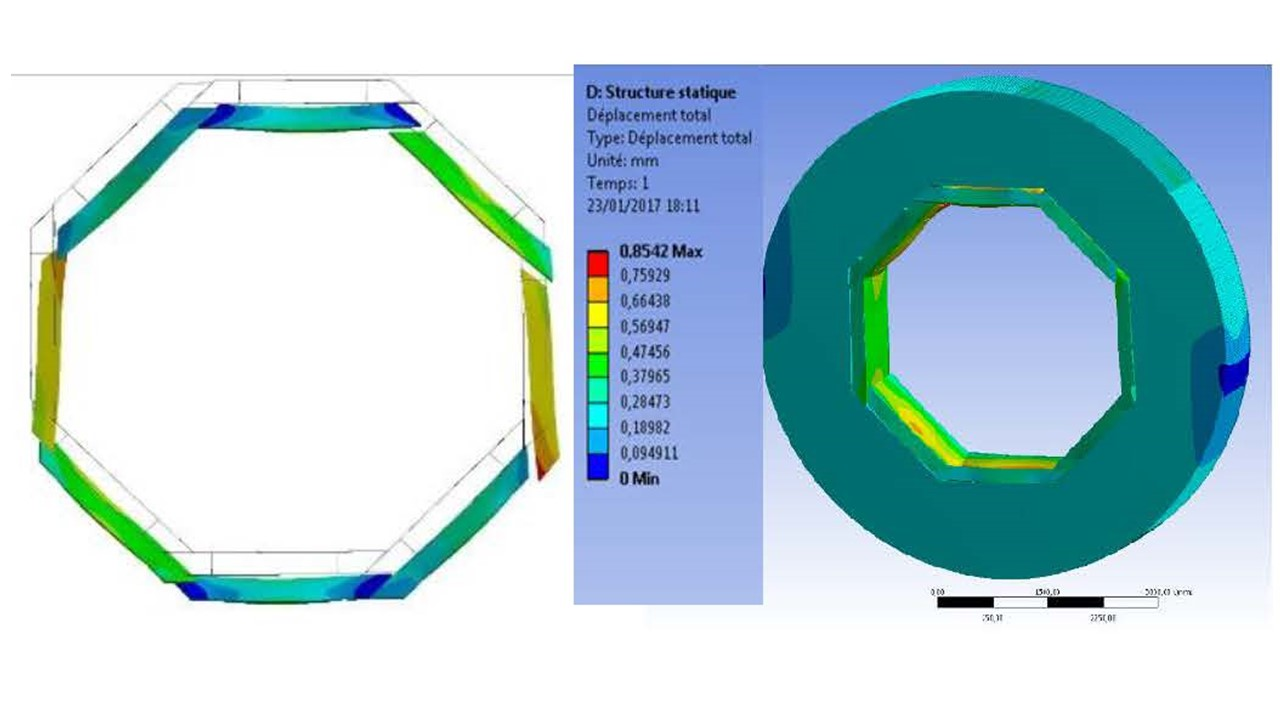
\includegraphics[width=1.0\hsize]{Integration/fig/Videau_deformations.jpg}
\caption{\label{fig:integration:Videau_deformations}Static deformations of the calorimeter "Videau" structure (right) and zoom on the electromagnetic modules displacements with a magnification factor of ??? (left).}
\end{figure}

\subparagraph{\textbf{TESLA simulations:}} \textit{Static and dynamic behaviour of TESLA structure}

\textit{Comment on LLR-DESY crosscheck.}

\subsection{Other subdetectors}

\textit{If available, results on the mechanical behaviour of other subdetectors (e.g. TPC) are also welcome.}

\vspace{2cm}
